\newpage
\section{Resultados}
	\subsection{Histograma}
		O cálculo do histograma é um procedimento simples, onde um vetor que contém a intensidade (luminância)  de cada pixel é indexado pelo valor do mesmo e incrementado a cada pixel.
		
		\begin{figure}[!htb]
			\centering
			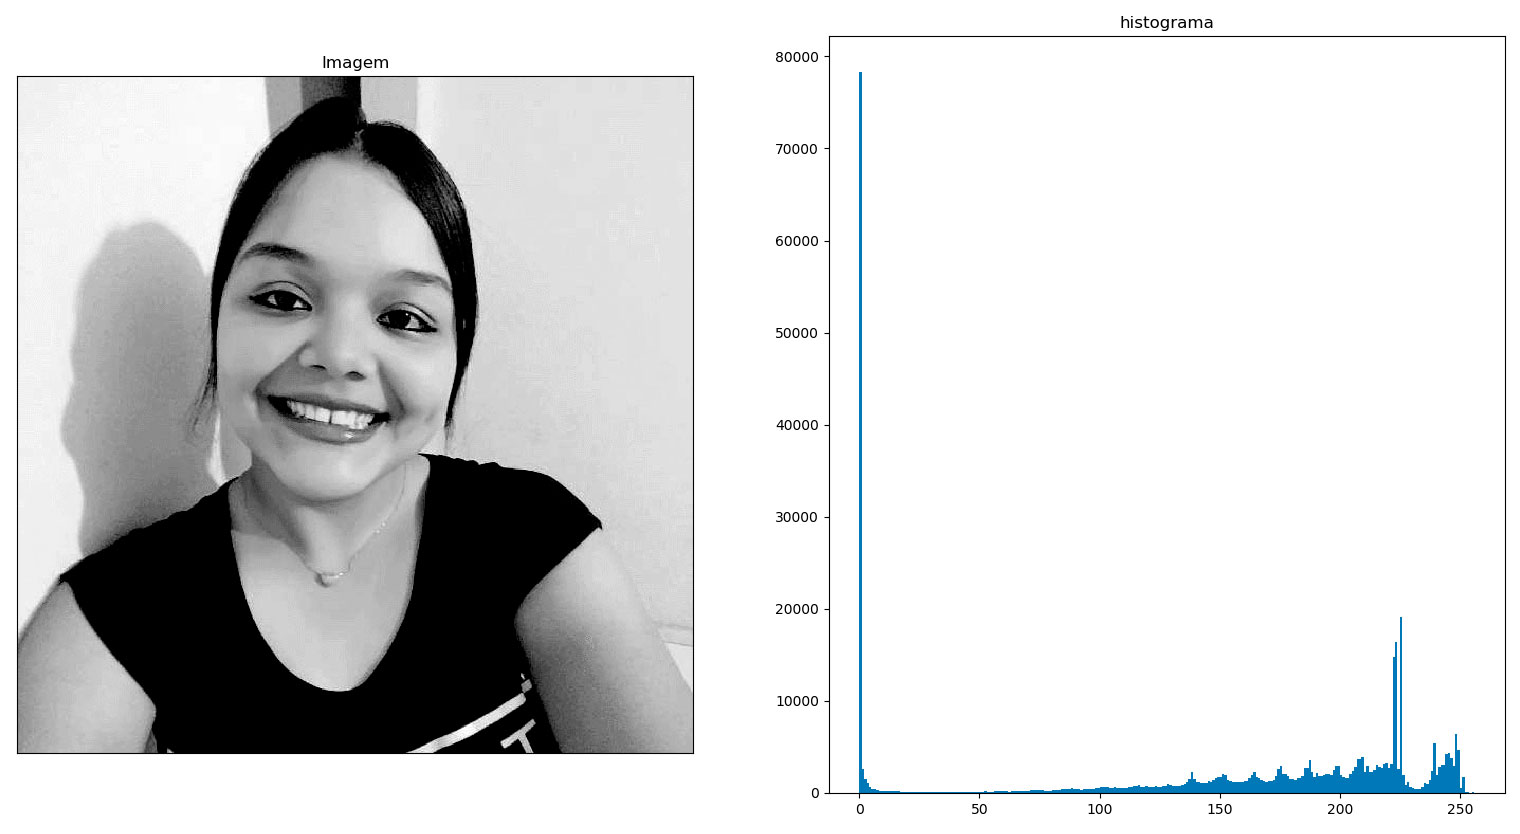
\includegraphics[width=\textwidth]{img/01-hist.jpg}
			\caption{Histograma da imagem}
		\end{figure}
	
		\lstset{language=c++}
		{\tiny \lstinputlisting{code/01-hist.cpp}}
		
	\subsection{Equalização do Histograma}
		O cálculo do histograma é um procedimento simples, onde um vetor que contém a intensidade (luminância)  de cada pixel é indexado pelo valor do mesmo e incrementado a cada pixel.
		
		\begin{figure}[!htb]
			\centering
			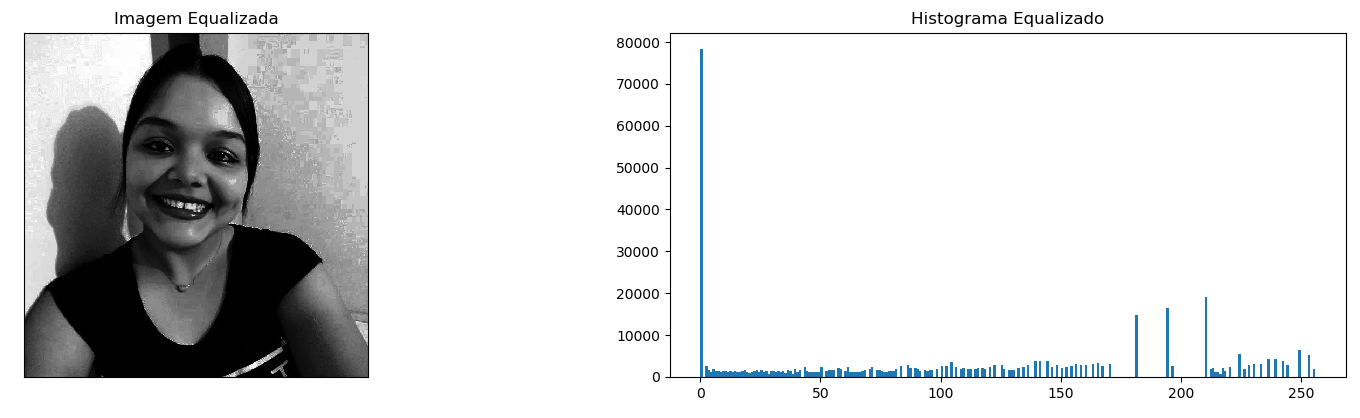
\includegraphics[width=\textwidth]{img/02-eq-hist.png}
			\caption{Histograma equalizado}
		\end{figure}
		
		\lstset{language=c++}
		{\tiny \lstinputlisting{code/02-eq-hist.cpp}}
		
	\subsection{Conversão para escala cinza}
		Algoritmo de escala de cinza baseado na luminosidade do pixel pela visão humana usando a fórmula: \texttt{L = R*0.3 + B*0.59 + G*0.11}. Dado o resultado o algoritmo salva o pixel na forma LLL. Primeiro convertemos a imagem em JPEG para PPM (formato simples e sem compressão, sendo mais fácil a manipulação), então obtemos um buffer dos pixels, na classe Image.
		
		\begin{figure}[!htb]
			\centering
			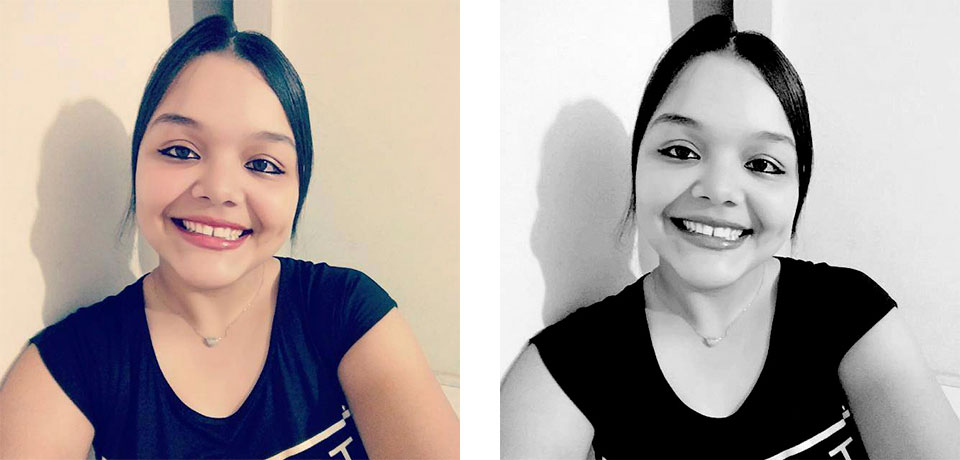
\includegraphics[width=\textwidth]{img/03-cinza.jpg}
			\caption{Imagem convertida para escala cinza}
		\end{figure}
		
		\lstset{language=Python}
		{\tiny \lstinputlisting{code/03-cinza.py}}
		
		\subsection{Rotacionamento de imagens}
			O método de rotação consiste em usar a matriz de pixel e deslocá-las de lugar como na imagem abaixo praticamente especificado.
			
			\begin{figure}[!htb]
				\centering
				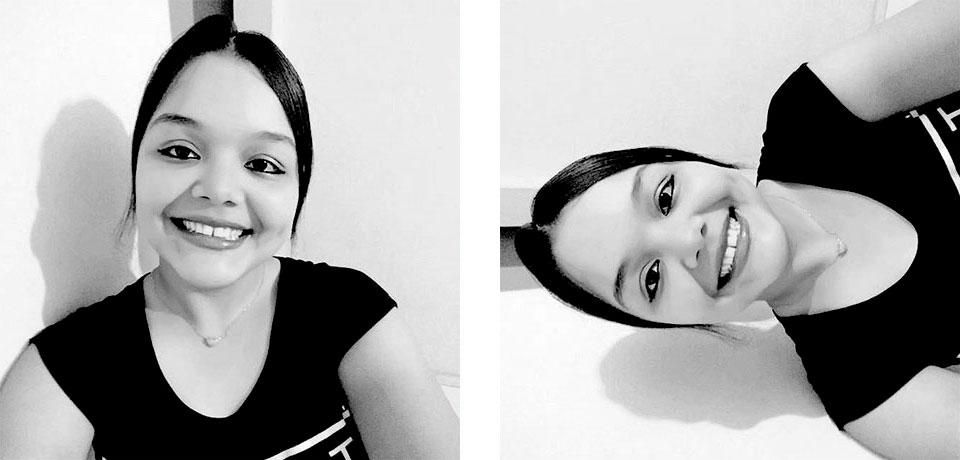
\includegraphics[width=\textwidth]{img/04-rotacao-1.jpg}
				\caption{Imagem rotacionada em sentido anti-horário}
			\end{figure}
			
			\begin{figure}[!htb]
					\centering
					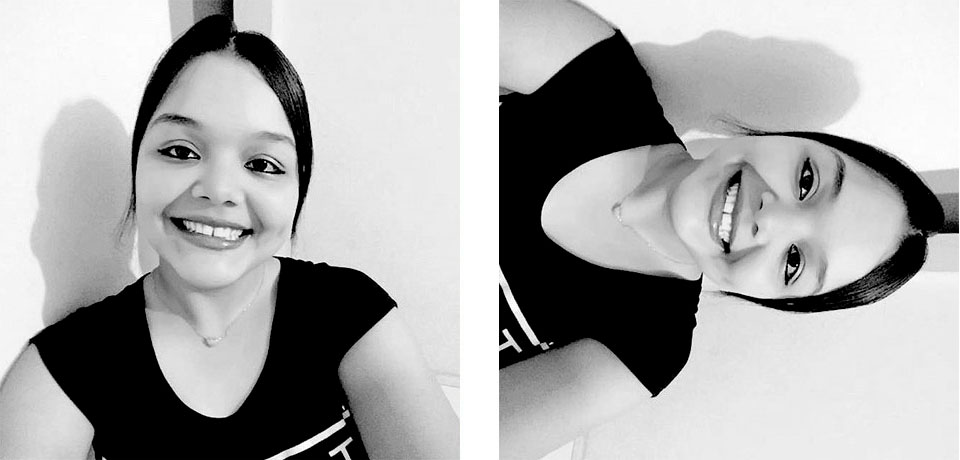
\includegraphics[width=\textwidth]{img/04-rotacao-2.jpg}
					\caption{Imagem rotacionada em sentido horário}
			\end{figure}
	
			\lstset{language=Python}
			{\tiny \lstinputlisting{code/04-rotacao.py}}
			
	\subsection{title}
		kkkk